\section{产品运营}
\subsection{产品简要介绍}\

\subsubsection{产品类型}\

全品类半开放式的知识付费平台——以教学视频以及配套音频,配套习题和配套资料为主。

\paragraph{全品类}\

单一品类竞争激烈,而且市场发展受限,而在线上教育领域并不存在所谓的“全部都做反而什么都做不好”的顾虑,因为平台只能做筛选教师工作,平台本身并不是知识的输出者,我们面向社会所有人招收教师来源,我们要做的是课程质量评价体系,保障课程质量,线上教育主要吸引人的是它便宜的价格。

\paragraph{半开放式}\

针对市面上已有的两种线上教育平台找老师的模式的综合与改进,一种是全开放式的,也就是拥有教师端的平台,平台通过对知识输出端的全开放,老师通过注册教师资格,自主上传教学课程;一种是全封闭式的,没有教师端,老师全靠课程运营联系,课程经审核规划后上线平台。

而半开放式平台是只开放教师联系的端口,老师不能直接上传课程,方便有知识变现需求的人联系平台,同时我们也要求课程运营联系老师,双管齐下,平台以此获取教师来源,从而筛选教师,教师需要遵守公司对课程录制的要求进行录课。
\vfill
% Table generated by Excel2LaTeX from sheet 'Sheet1'
\begin{table}[H]
  \centering
  \caption{运营模式对比}
    \begin{tabular}{|r|p{8.89em}|c|}
    \hline
    \textcolor[rgb]{ .298,  .282,  .239}{} & \textcolor[rgb]{ .298,  .282,  .239}{优点} & \multicolumn{1}{p{14.055em}|}{\textcolor[rgb]{ .298,  .282,  .239}{缺点}} \\
    \hline
    \multicolumn{1}{|r|}{\multirow{4}[2]{*}{\textcolor[rgb]{ .298,  .282,  .239}{全开放式平台}}} & \multirow{4}[2]{*}{\textcolor[rgb]{ .298,  .282,  .239}{课程覆盖速度快}} & \multicolumn{1}{p{14.055em}|}{\textcolor[rgb]{ .298,  .282,  .239}{1.管理混乱}} \\
          & \multicolumn{1}{c|}{} & \multicolumn{1}{p{14.055em}|}{\textcolor[rgb]{ .298,  .282,  .239}{2.课程质量很难保障}} \\
          & \multicolumn{1}{c|}{} & \multicolumn{1}{p{14.055em}|}{\textcolor[rgb]{ .298,  .282,  .239}{3.平台后期知识管理实施困难}} \\
          & \multicolumn{1}{c|}{} & \multicolumn{1}{p{14.055em}|}{\textcolor[rgb]{ .298,  .282,  .239}{4.课程盈利较少,只是抽取平台使用费}} \\
    \hline
    \multicolumn{1}{|r|}{\multirow{3}[2]{*}{\textcolor[rgb]{ .298,  .282,  .239}{全封闭式平台}}} & \textcolor[rgb]{ .298,  .282,  .239}{1.课程质量平台可控制} & \multicolumn{1}{p{14.055em}|}{\textcolor[rgb]{ .298,  .282,  .239}{1.效率低}} \\
          & \textcolor[rgb]{ .298,  .282,  .239}{2.后期知识管理方便} & \multicolumn{1}{p{14.055em}|}{\textcolor[rgb]{ .298,  .282,  .239}{2.课程制作周期长}} \\
          & \textcolor[rgb]{ .298,  .282,  .239}{3.课程盈利较多} & \multicolumn{1}{p{14.055em}|}{\textcolor[rgb]{ .298,  .282,  .239}{3.课程覆盖速度慢}} \\
    \hline
    \multicolumn{1}{|r|}{\multirow{5}[2]{*}{\textcolor[rgb]{ .298,  .282,  .239}{半开放式平台}}} & \textcolor[rgb]{ .298,  .282,  .239}{1.课程质量平台可控制} & \multicolumn{1}{c|}{\multirow{5}[2]{*}{\textcolor[rgb]{ .298,  .282,  .239}{暂无}}} \\
          & \textcolor[rgb]{ .298,  .282,  .239}{2.后期知识管理方便} &  \\
          & \textcolor[rgb]{ .298,  .282,  .239}{3.课程制作周期短} &  \\
          & \textcolor[rgb]{ .298,  .282,  .239}{4.课程覆盖速度快} &  \\
          & \textcolor[rgb]{ .298,  .282,  .239}{5.课程盈利较多} &  \\
    \hline
    \end{tabular}%
  \label{tab:yymsdb}%
\end{table}%


\subsubsection{产品核心}\

课程内容为核心,技术为工具。

前期通过与老师签订版权归属协议,拥有对高等教育高质量的、公司具有完全版权的课程,后期通过对课程的二次加工,整合课程,对现有知识形成一个知识创造。给用户个性化推荐课程套餐,而这种课程二次加工后的课程套餐,对于拥有课程完全版权的公司来说成本低且易操作。

\subsubsection{产品市场切入点}\

K12之后的线上教育。如:

成人教育:信息技术;平面设计;

高等教育:高等数学;

技能培训:化妆课;插花;

资格考试:司法考试;公务员考试。

原因:首先是因为K12已经有了行业巨头与行业标准(学而思),其次是考虑到对社会的影响来说,真正助推中国社会对人才的需求的,不是K12,而是成人教育。但另一方面,我们并不是完全放弃K12,我们是全品类的知识付费平台,为了迎合市场刚需和与政府的合作,平台的课程课程将会覆盖到K12,在这方面的课程质量保障,只需要直接联系学而思现役有经验的老师录制课程,然后我们以较低价格提供给市场或者免费送课(价格战)。

\subsection{课程运营选择方向}
\subsubsection{录课形式}\

作为全品类的平台,全品类不仅体现在课程种类上,也体现在录课形式上,主要分为两种录课形式。举现有的市场平台的例子,万题库,它是只做直播课程的全开放平台,但直播课并没有达到预期的效果,甚至还不如录播课,参考艾瑞咨询:2018年1月中国在线教育平台用户大数据报告:腾讯课堂数据篇

\begin{figure}[H]
	\centering
	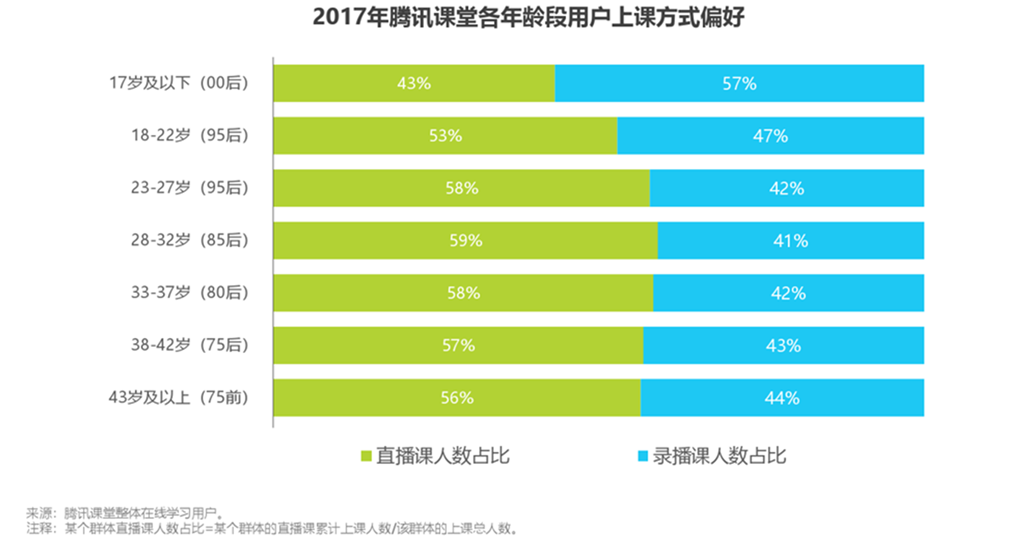
\includegraphics[width=0.9\columnwidth]{figures/tecent_couse.png}
	%  \setlength{\abovecaptionskip}{0pt}
	%  \setlength{\belowcaptionskip}{-20pt}
	\caption{2017年腾讯课堂各年龄用户上课方式偏好}
	\label{fg:tecent_couse}
\end{figure}

这张图我们可以看到,并不是像万题库所描述的那样,直播课对于录播课来说具有压倒性优势,所以只做直播课就好了,而是我们看到越年轻的人群越喜欢录播课,他们更适应快捷的获取知识的方式,对他们来说直播听课花费的时间太高。另一方面,直播课还存在很多问题,比如现阶段直播间的普遍问题,主播有事暂离,只能空闲等待,在直播课时,若老师临时演板,也就只能等老师写完,这段时间是接受知识的空白区。老师语速慢也不能快进,在时间上效率较低。而且直播所推崇的实时互动只局限于小用户量,人数一旦达到一定数量,实时互动的效果就会大打折扣。所以,直播课和录播课我们都要有,直播课有它在学习效果上的优势,而录播课则也有它受欢迎的人群。对于市场需求来说二者相对平均,这在某种程度上再一次验证了坚持全品类的正确性。

\subsubsection{课程内容}\

\paragraph{市场受欢迎的课}\

作为商业公司,首先以盈利为主,公司的前期的成本回收主要依靠于此。公司将会在课程选择前做好市场调查,而市场调查的主要手段包括各数据平台年报数据分析,与对业内人生访谈,对知乎的调研。

\paragraph{为形成公司完整课程体系的课}\

为了提高公司的竞争潜力与核心竞争力,需要尽快完善课程体系,首先遍历大学大类课程,比如经济金融课程体系化特训班,拿到完全版权后,课程将被按大学课程拆分成微观经济学部分,宏观经济学部分等单独售卖,之后通过销售反馈销售情况,再考虑是否就受欢迎课程进行重新录制,提高该类课程质量。当公司大量盈利之后将遍历精细化所有小门类课程,以做出品牌效应。

\paragraph{为和政府合作提高社会影响力的课}\

首选K12.。

\subsubsection{其他非视频形式}\

\paragraph{课程配套资料}\

课程配套资料,可以通过学生自己上传,公司整理后可出书出售。

\paragraph{课程音频}\

为了满足部分课程内容对于图像资料的需求度不高,和部分用户有只听音频的需求,公司的课程需要有单独的音频部分可以供用户体验。

\paragraph{课程配套习题}\

后期上线的功能,主要在于评价学生知识掌握情况,与后期习题册出版。

\subsection{课程制作流程图}
课程制作流程如下:
\begin{figure}[H]
	\centering
	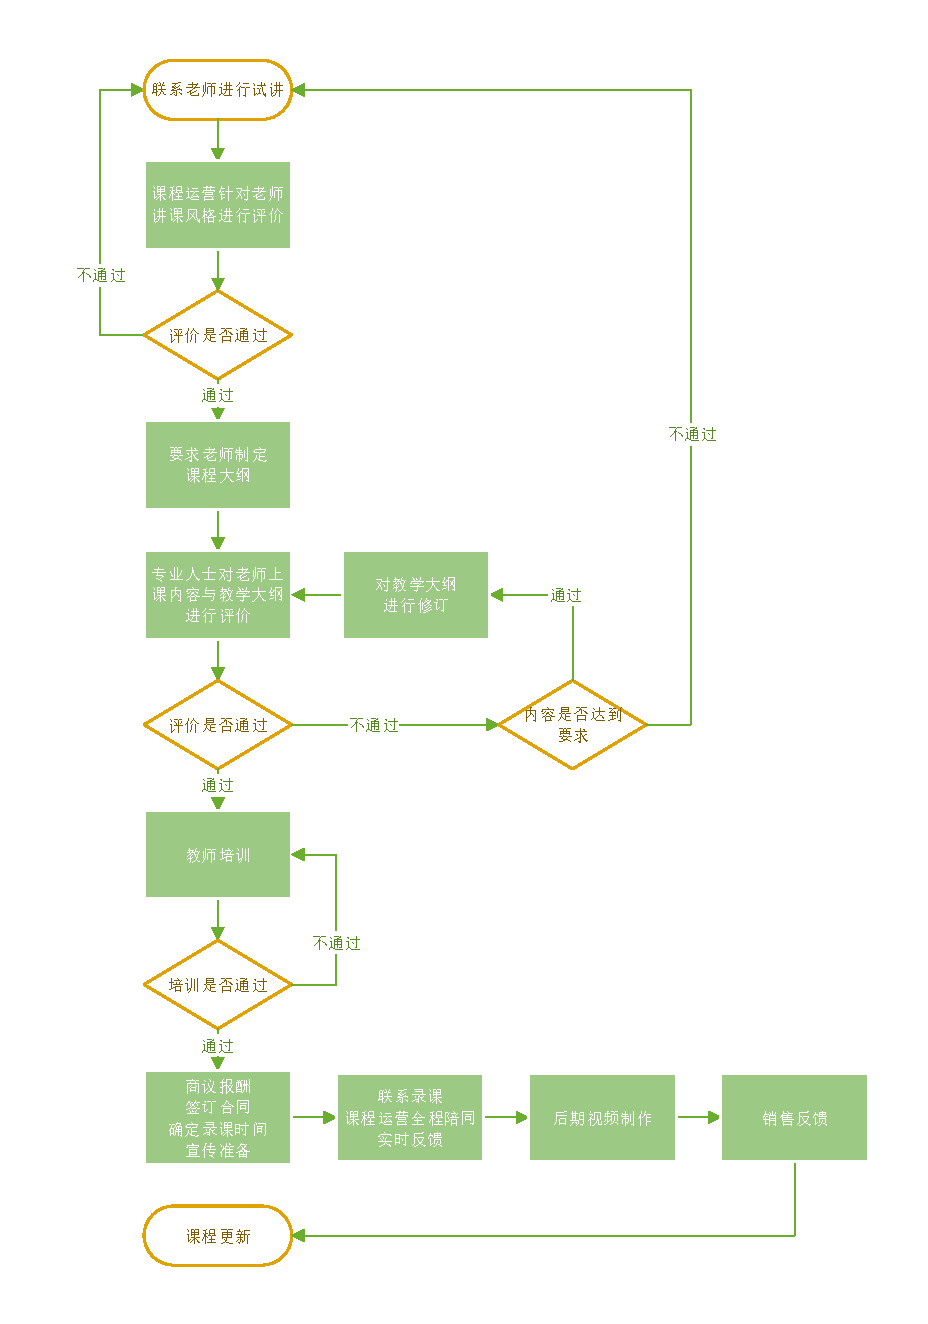
\includegraphics[width=0.9\columnwidth]{figures/couse_process}
	%  \setlength{\abovecaptionskip}{0pt}
	%  \setlength{\belowcaptionskip}{-20pt}
	\caption{课程制作流程图}
	\label{fg:couse_process}
\end{figure}

\subsection{课程功能实现}\

\paragraph{奖励机制}\

通过用户课程笔记的上传,后台会评价出最优的笔记,分享给所有的用户,上传者该课程免费。

\paragraph{评价系统}\

点赞量高、内容质量好的评价会优先显示在顶端(参考网易云音乐的评价系统)。

\paragraph{学友系统(后期可以考虑实现)}\

学生之间可以加好友加关注,一起学习,互相留言探讨问题,也相当于借鉴现在软件系统行业发展的趋势,社交是用户黏度的另一种提升方式。参考各类游戏、实用软件,大部分都植入了社交系统,因为人是群居动物,具有随大流的趋势。

\paragraph{答疑系统,师生交互(成熟后实现)}\

可选取专门时间段开教师直播答疑课,解决学员在学习过程中遇到的典型性问题。问题来源可以是专门学员反馈(课后留专门邮箱接收),也可以是讨论区(类似学友系统)反馈,也可以是老师想到的典型问题。

\subsection{课程质量控制}
\subsubsection{课程分类体系}\

初步方案:

\begin{figure}[H]
	\centering
	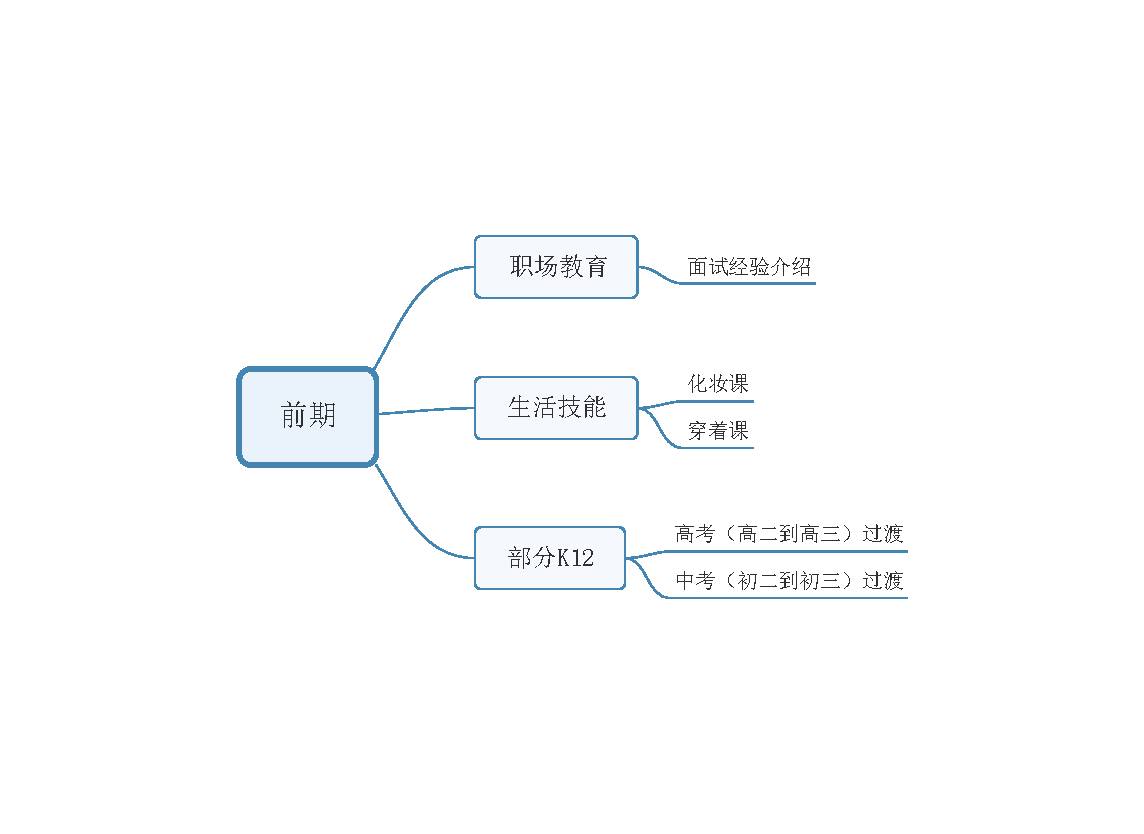
\includegraphics[width=0.9\columnwidth]{figures/prophase_development}
	%  \setlength{\abovecaptionskip}{0pt}
	%  \setlength{\belowcaptionskip}{-20pt}
	\caption{课程分类体系}
	\label{fg:prophase_development}
\end{figure}

最终方案:参考第一章第7节第2小节长期目标图\ref{fg:aft_development}

\subsubsection{教师来源}\

\paragraph{老师客户}\

在平台主动联系公司的老师,这也是公司主要想发展的方面,前期通过宣传,长期通过做口碑来实现这一点。

\paragraph{高校学生}\

公司的创业团队覆盖了北京最好的几所高校,据我们了解,我们身边想要知识变现的人很多,公司可以直接通过公司管理层或者员工联系同学校的学生资源。使用我们创业团队的优势,收集北京各个院校的各个学院的情况,找到有空余时间的学生。另一方面,对于学生来说公司可以给于的报酬足够吸引他们来将知识变现。而阻碍合作的有两个主要的原因,一是没有时间,二是路程。

\paragraph{线下机构教师}\

成熟机构有经验的老师,技能培训以及从业资格考试类。

\subsubsection{教师要求}\

\paragraph{试讲环节}\

试讲评分项目:
% Table generated by Excel2LaTeX from sheet 'Sheet1'
\begin{table}[H]
  \centering
  \caption{试讲评分项目}
    \begin{tabular}{|p{16.165em}|r|}
    \hline
    \textcolor[rgb]{ .298,  .282,  .239}{试讲评分项目} & \multicolumn{1}{p{16.945em}|}{\textcolor[rgb]{ .298,  .282,  .239}{分数(10分制)}} \\
    \hline
    \textcolor[rgb]{ .298,  .282,  .239}{1.所讲内容是否正确(基础)} & \textcolor[rgb]{ .298,  .282,  .239}{} \\
    \hline
    \textcolor[rgb]{ .298,  .282,  .239}{2.语速是否适当} & \textcolor[rgb]{ .298,  .282,  .239}{} \\
    \hline
    \textcolor[rgb]{ .298,  .282,  .239}{3.讲课逻辑是否清晰} & \textcolor[rgb]{ .298,  .282,  .239}{} \\
    \hline
    \textcolor[rgb]{ .298,  .282,  .239}{4.习惯语是否太多,呃嗯等} & \textcolor[rgb]{ .298,  .282,  .239}{} \\
    \hline
    \textcolor[rgb]{ .298,  .282,  .239}{5.是否用太多的专业术语让人不好理解} & \textcolor[rgb]{ .298,  .282,  .239}{} \\
    \hline
    \textcolor[rgb]{ .298,  .282,  .239}{6.准备是否充分,知道自己接下来要讲什么} & \textcolor[rgb]{ .298,  .282,  .239}{} \\
    \hline
    \textcolor[rgb]{ .298,  .282,  .239}{7.声音是否洪亮} & \textcolor[rgb]{ .298,  .282,  .239}{} \\
    \hline
    \textcolor[rgb]{ .298,  .282,  .239}{8.录课形象是否合适} & \textcolor[rgb]{ .298,  .282,  .239}{} \\
    \hline
    \end{tabular}%
  \label{tab:sjpfxm}%
\end{table}%


\paragraph{第三方评价环境}\

讲课内容评价
% Table generated by Excel2LaTeX from sheet 'Sheet1'
\begin{table}[H]
  \centering
  \caption{讲课内容评价}
    \begin{tabular}{|p{14.335em}|r|}
    \hline
    \textcolor[rgb]{ .298,  .282,  .239}{讲课内容具体评价} & \multicolumn{1}{p{12.665em}|}{\textcolor[rgb]{ .298,  .282,  .239}{分数(10分制)}} \\
    \hline
    \textcolor[rgb]{ .298,  .282,  .239}{1.所讲内容是否正确(专业角度)} & \textcolor[rgb]{ .298,  .282,  .239}{} \\
    \hline
    \textcolor[rgb]{ .298,  .282,  .239}{2.所讲知识是否足够前沿} & \textcolor[rgb]{ .298,  .282,  .239}{} \\
    \hline
    \textcolor[rgb]{ .298,  .282,  .239}{3.教学大纲内容设计是否合理} & \textcolor[rgb]{ .298,  .282,  .239}{} \\
    \hline
    \textcolor[rgb]{ .298,  .282,  .239}{4.教学大纲时间分配是否得当} & \textcolor[rgb]{ .298,  .282,  .239}{} \\
    \hline
    \textcolor[rgb]{ .298,  .282,  .239}{5.作为专业学生,您是否想听他/她的课} & \textcolor[rgb]{ .298,  .282,  .239}{} \\
    \hline
    \end{tabular}%
  \label{tab:nrpf}%
\end{table}%


\subsubsection{教师合同}\

教学兼职合同

录播教学课程合同/直播教学课程合同

版权归属协议(许可使用作品目录)

买断教师一定时间内线上同类型课程录制权利

\subsubsection{课程制作周期}\
以微观经济学为例:
% Table generated by Excel2LaTeX from sheet 'Sheet1'
\begin{table}[H]
  \centering
  \caption{课程更新周期(例)}
    \begin{tabular}{|p{5.165em}|p{6.61em}|p{8.165em}|p{4.055em}|}
    \hline
    \textcolor[rgb]{ .298,  .282,  .239}{课程类型} & \textcolor[rgb]{ .298,  .282,  .239}{课程名称} & \textcolor[rgb]{ .298,  .282,  .239}{一年内是否需要更新} & \textcolor[rgb]{ .298,  .282,  .239}{更新周期} \\
    \hline
    \textcolor[rgb]{ .298,  .282,  .239}{大学专业课} & \textcolor[rgb]{ .298,  .282,  .239}{微观经济学} & \textcolor[rgb]{ .298,  .282,  .239}{否} & \textcolor[rgb]{ .298,  .282,  .239}{2-3年} \\
    \hline
    \end{tabular}%
  \label{tab:kcgxzq}%
\end{table}%


\subsection{成本投入}
\subsubsection{兼职教师报酬}\

兼职教师报酬为:
% Table generated by Excel2LaTeX from sheet 'Sheet1'
\begin{table}[H]
  \centering
  \caption{兼职教师报酬}
    \begin{tabular}{|p{5.165em}|p{8.665em}|p{6.835em}|p{5.5em}|}
    \hline
    \textcolor[rgb]{ .298,  .282,  .239}{教师类型} & \textcolor[rgb]{ .298,  .282,  .239}{讲课内容} & \textcolor[rgb]{ .298,  .282,  .239}{形式} & \textcolor[rgb]{ .298,  .282,  .239}{价格} \\
    \hline
    \textcolor[rgb]{ .298,  .282,  .239}{大学博士} & \textcolor[rgb]{ .298,  .282,  .239}{高等教育、司法考试} & \textcolor[rgb]{ .298,  .282,  .239}{直播+录播} & \textcolor[rgb]{ .298,  .282,  .239}{1000+/h} \\
    \hline
    \textcolor[rgb]{ .298,  .282,  .239}{大学硕士} & \textcolor[rgb]{ .298,  .282,  .239}{高等教育、考研、基础课程} & \textcolor[rgb]{ .298,  .282,  .239}{教研+直播+录播} & \textcolor[rgb]{ .298,  .282,  .239}{400-1000/h} \\
    \hline
    \textcolor[rgb]{ .298,  .282,  .239}{大学本科} & \textcolor[rgb]{ .298,  .282,  .239}{K12} & \textcolor[rgb]{ .298,  .282,  .239}{录播} & \textcolor[rgb]{ .298,  .282,  .239}{500/h} \\
    \hline
    \textcolor[rgb]{ .298,  .282,  .239}{社会人士} & \textcolor[rgb]{ .298,  .282,  .239}{公务员考试、化妆课;兴趣课技能课考证课} & \textcolor[rgb]{ .298,  .282,  .239}{录播} & \textcolor[rgb]{ .298,  .282,  .239}{1000/h} \\
    \hline
    \end{tabular}%
  \label{tab:jzlsbc}%
\end{table}%


\subsubsection{场地需求}\

\paragraph{直播课场地}\

场地要求:
\begin{itemize}
  \item 场地大小:20平米
  \item 录课环境安静(必要时贴吸音泡沫)
  \item 录课时空调声音不能影响录课效果
\end{itemize}


\paragraph{录播课场地}\

场地要求:
\begin{itemize}
  \item 场地大小:5-6平米
  \item 录课环境安静(必要时贴吸音泡沫)
  \item 录课时空调声音不能影响录课效果
\end{itemize}


\paragraph{办公场地}\

场地要求:
\begin{itemize}
  \item 离录课间足够近,随时反馈问题
  \item 可长期使用
\end{itemize}


\subsubsection{设备需求}\

场地和设备成本预算为79799元


\subsection{版权保护}
视频加水印,课程资料加水印,合同在法律上保障公司对课程的永久版权。












